\documentclass[11pt]{article}
\input{../calcnotes.sty}
\fancyhead[C]{1.6 Trigonometric Functions}

\begin{document}

\noindent What's a radian? Why do we use it?\\[2ex]

\noindent Find the length of an arc subtended on a circle of radius $\displaystyle 3$ by a central angle of measure $\displaystyle \frac{2\pi}{3}$.\\[2ex]

\noindent Remember this? I hope so\dots\\[1ex]

\begin{center}
    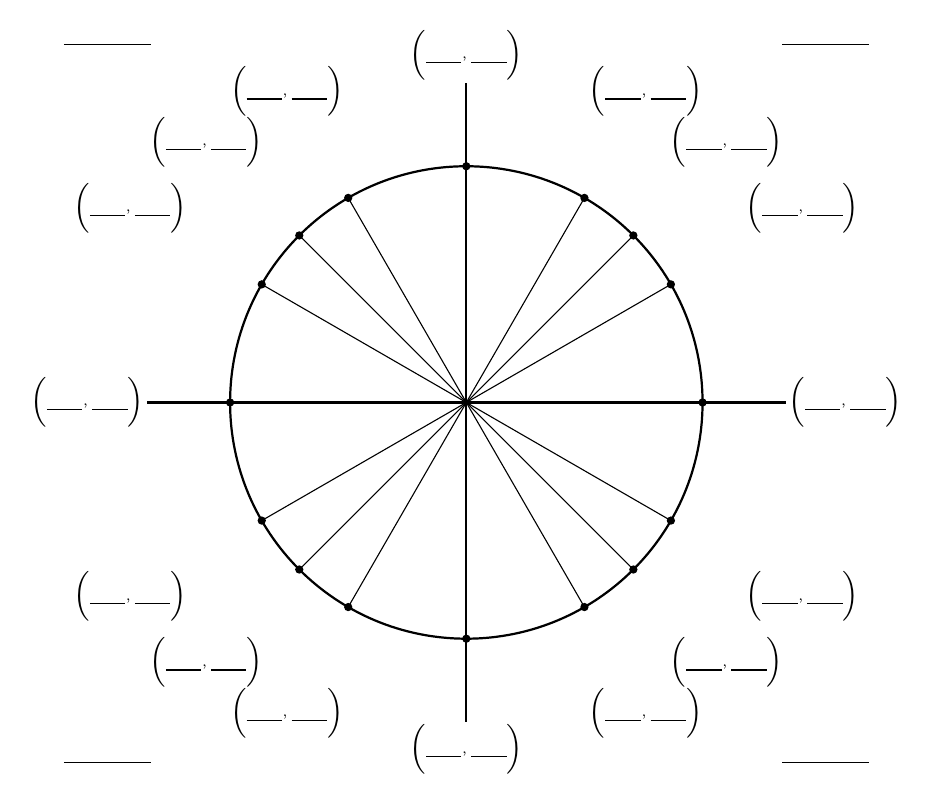
\begin{tikzpicture}[scale=3.0]
        \draw[thick, black!70!black] (0,0) circle(1);
        \draw[->, black!80!black, thick] (-1.45,0) -- (1.45,0);
        \draw[->, black!80!black, thick] (0,-1.45) -- (0,1.45);

        \foreach \a in {30,45,60,120,135,150,210,225,240,300,315,330} {
                \draw[black!80!black, thin] (0,0) -- (\a:1);
                \fill[black!80!black] (\a:1) circle(0.5pt);
                \pgfmathtruncatemacro{\opp}{mod(\a+180,360)}
                \node[anchor=\opp, font=\tiny] at (\a:1.35)
                {$\bigl(\underline{\hspace{0.45cm}},\underline{\hspace{0.45cm}}\bigr)$};
            }

        \draw[black!80!black, thin] (0,0) -- (1,0);
        \fill[black!80!black] (1,0) circle(0.5pt);
        \node[anchor=west, font=\tiny, fill=white, inner sep=1pt] at (1.35, 0)
        {$\bigl(\underline{\hspace{0.45cm}},\underline{\hspace{0.45cm}}\bigr)$};

        \draw[black!80!black, thin] (0,0) -- (0,1);
        \fill[black!80!black] (0,1) circle(0.5pt);
        \node[anchor=south, font=\tiny, fill=white, inner sep=1pt] at (0, 1.35)
        {$\bigl(\underline{\hspace{0.45cm}},\underline{\hspace{0.45cm}}\bigr)$};

        \draw[black!80!black, thin] (0,0) -- (-1,0);
        \fill[black!80!black] (-1,0) circle(0.5pt);
        \node[anchor=east, font=\tiny, fill=white, inner sep=1pt] at (-1.35, 0)
        {$\bigl(\underline{\hspace{0.45cm}},\underline{\hspace{0.45cm}}\bigr)$};

        \draw[black!80!black, thin] (0,0) -- (0,-1);
        \fill[black!80!black] (0,-1) circle(0.5pt);
        \node[anchor=north, font=\tiny, fill=white, inner sep=1pt] at (0, -1.35)
        {$\bigl(\underline{\hspace{0.45cm}},\underline{\hspace{0.45cm}}\bigr)$};

        \node[font=\tiny] at ( 1.52,  1.52) {$\underline{\hspace{1.1cm}}$};
        \node[font=\tiny] at (-1.52,  1.52) {$\underline{\hspace{1.1cm}}$};
        \node[font=\tiny] at (-1.52, -1.52) {$\underline{\hspace{1.1cm}}$};
        \node[font=\tiny] at ( 1.52, -1.52) {$\underline{\hspace{1.1cm}}$};
    \end{tikzpicture}\\[1ex]

    $\cos \longrightarrow \underline{\hspace{1.5cm}}$ \hspace{4cm} $\displaystyle \sin \longrightarrow \underline{\hspace{1.5cm}}$
\end{center}

\noindent Write an angle $\displaystyle \theta$ in standard position on a circle of radius $\displaystyle r$ and find the six basic trig functions at that point.\\[2ex]

\newpage

\noindent Graph all six basic trig functions below. Which are even? Odd? Neither?

\begin{center}
    \begin{minipage}{0.32\textwidth}
        \centering $\displaystyle y = \sin x$\\[3pt]
        \smallgraph
    \end{minipage}
    \begin{minipage}{0.32\textwidth}
        \centering $\displaystyle y = \cos x$\\[3pt]
        \smallgraph
    \end{minipage}
    \begin{minipage}{0.32\textwidth}
        \centering $\displaystyle y = \tan x$\\[3pt]
        \smallgraph
    \end{minipage}

    \vspace{1ex}

    \begin{minipage}{0.32\textwidth}
        \centering $\displaystyle y = \csc x$\\[3pt]
        \smallgraph
    \end{minipage}
    \begin{minipage}{0.32\textwidth}
        \centering $\displaystyle y = \sec x$\\[3pt]
        \smallgraph
    \end{minipage}
    \begin{minipage}{0.32\textwidth}
        \centering $\displaystyle y = \cot x$\\[3pt]
        \smallgraph
    \end{minipage}
\end{center}

\vspace{1ex}

\noindent What is the period for the six basic trig functions? How do we define period?\\[2ex]

\noindent Here are some problems to try:

\begin{enumerate}
    \item Find all of the trig values of $\displaystyle \theta$ if $\displaystyle \sin \theta = \frac{-3}{5}$ and $\displaystyle \tan \theta < 0$.\\[2ex]

    \item Graph $\displaystyle y = 3\cos\!\left(2\left(x-\frac{\pi}{2}\right)\right) + 1$. Label the period, amplitude, domain, range, and shifts.

          \emptygraph
\end{enumerate}

\vspace{2ex}

\noindent And now the hard stuff (ha!). What does $\displaystyle \cos^{-1}(-0.5)$ mean?\\[2ex]

\newpage

\noindent Can we use any spot on the unit circle? Why or why not? Is there a difference between that question and solving $\displaystyle \cos(x) = -0.5$?\\[2ex]

\noindent What are the domain and range for the inverse trig functions?\\[2ex]

\noindent Can you graph them?

\begin{center}
    \begin{minipage}{0.32\textwidth}
        \centering $\displaystyle y = \sin^{-1} x$\\[3pt]
        \smallgraph
    \end{minipage}
    \begin{minipage}{0.32\textwidth}
        \centering $\displaystyle y = \cos^{-1} x$\\[3pt]
        \smallgraph
    \end{minipage}
    \begin{minipage}{0.32\textwidth}
        \centering $\displaystyle y = \tan^{-1} x$\\[3pt]
        \smallgraph
    \end{minipage}
\end{center}

\end{document}
